\section{Teorema de Ceva y Menelao}

\begin{sol}
	Note que por la propiedad de tangencia del inc\'irculo, tenemos $BZ =BX$, $CX = CY$, $AY = AZ$. Por lo tanto $\frac{AZ}{ZB}\cdot \frac{BX}{CX} \cdot \frac{CY}{AY} = 1$ y por lo tanto las tres cevianas concurren
\end{sol}

\begin{sol}
	Observe que las seis sumas dadas en el problema todas suman igual al semiper\'imetro del tri\'angulo. Por eso, Tenemos por ejemplo que $AB+BL = AB + AM \implies BL = AM$. Analogamente $AN = LC y BN = MC$. Por lo tanto $\frac{AN}{BN}\cdot \frac{BL}{CL} \cdot \frac{CM}{AM} = 1$ y los puntos concurren.
\end{sol}

\begin{sol}
	\begin{lem}
		$BFD \simeq BCA$:
	\end{lem}
	\textit{Prueba:} Sea $H$ el ortocentro. Como $\angle{CFB} = 90^{\circ} = \angle{ADB} \implies  HFBD $ es un cuadril\'atero c\'iclico. Entonces $\angle{DFB} =\angle{BHD} = \angle{AHE} = 90^{\circ} - \angle {HAC} = \angle{BCA}$. An\'alogamente, $\angle{BAC } = \angle{BDF}$. el resultado sigue por el criterio AAA. $\square$
	
	Ahora, como $BQ$ es altura de $BFD$, mas el lemma anterior podemos concluir que $\angle{QBF} = \angle{EBD}, \angle{QBD} = \angle{EBA}$. (Usando el hecho de que $BE$ tambi\'en es altura). Por lo tanto, usando el teorema de ceva trigonom\'etrico:
	\begin{equation}
	\frac{\sin{\angle{ABQ}}}{\sin{\angle{QBC}}} \cdot\frac{\sin{\angle{BCR}}}{\sin{\angle{RCA}}} \cdot\frac{\sin{\angle{CAP}}}{\sin{\angle{PAB}}} = \frac{\sin{\angle{CBE}}}{\sin{\angle{ABE}}} \cdot\frac{\sin{\angle{FCA}}}{\sin{\angle{FCB}}} \cdot\frac{\sin{\angle{BAD}}}{\sin{\angle{DAC}}} = 1
	\end{equation}
	Debido a que las alturas de $ABC$ concurren en $H$ (Vuelta de Teorema de Ceva)
\end{sol}

\begin{sol}
	Solucion en proceso
\end{sol}

\begin{sol}
	Vea que $AV$ es el di\'ametro de la circunferencia (ver \ref{fig1}), puesto que $\angle{AHV} = 90^{\circ}$. Eso significa que $\angle{VEA} = \angle{VFA} = 90^{\circ}$. Usando eso + AAA concluimos que los tri\'angulos $AVF$ y $AVE$ son congruentes. Es particular, $AF = AE \label{Eq4}$.
	\begin{align}
	BD \cdot BV &= BF \cdot BA \label{Eq1} \\ 
	CV \cdot CD & = CE \cdot CA \label{Eq2} \\ 
	\frac{AB}{AC} & = \frac{BV}{VC} \label{Eq3}
	\end{align}
	La ecuaci\'on \ref{Eq1} Sigue de usar potencia de un punto alrededor de B. La ecuaci\'on \ref{Eq2} sigue de usar potencia de un punto alrededor de A, y la ecuaci\'on \ref{Eq3} sigue del teorema de la bisectriz.
	
	Dividiendo \ref{Eq1} entre \ref{Eq2}, y usando \ref{Eq3} nos da
	\begin{align}
	\frac{BF \cdot BA }{CE \cdot CA} = \frac{BD \cdot BV}{CV \cdot CD} \implies \frac{BF\cdot CD}{CE\cdot DB} = \frac{AC\cdot BV}{AB\cdot VC} = 1
	\end{align}
	En otras palabras, usando $AF = AE$.
	\begin{align}
	\frac{BF\cdot CD \cdot AE}{CE\cdot DB \cdot AF} = 1 \implies AD, BE, CF son colineales.
	\end{align}
	\begin{figure}[h!] \label{fig1}
		\centering
		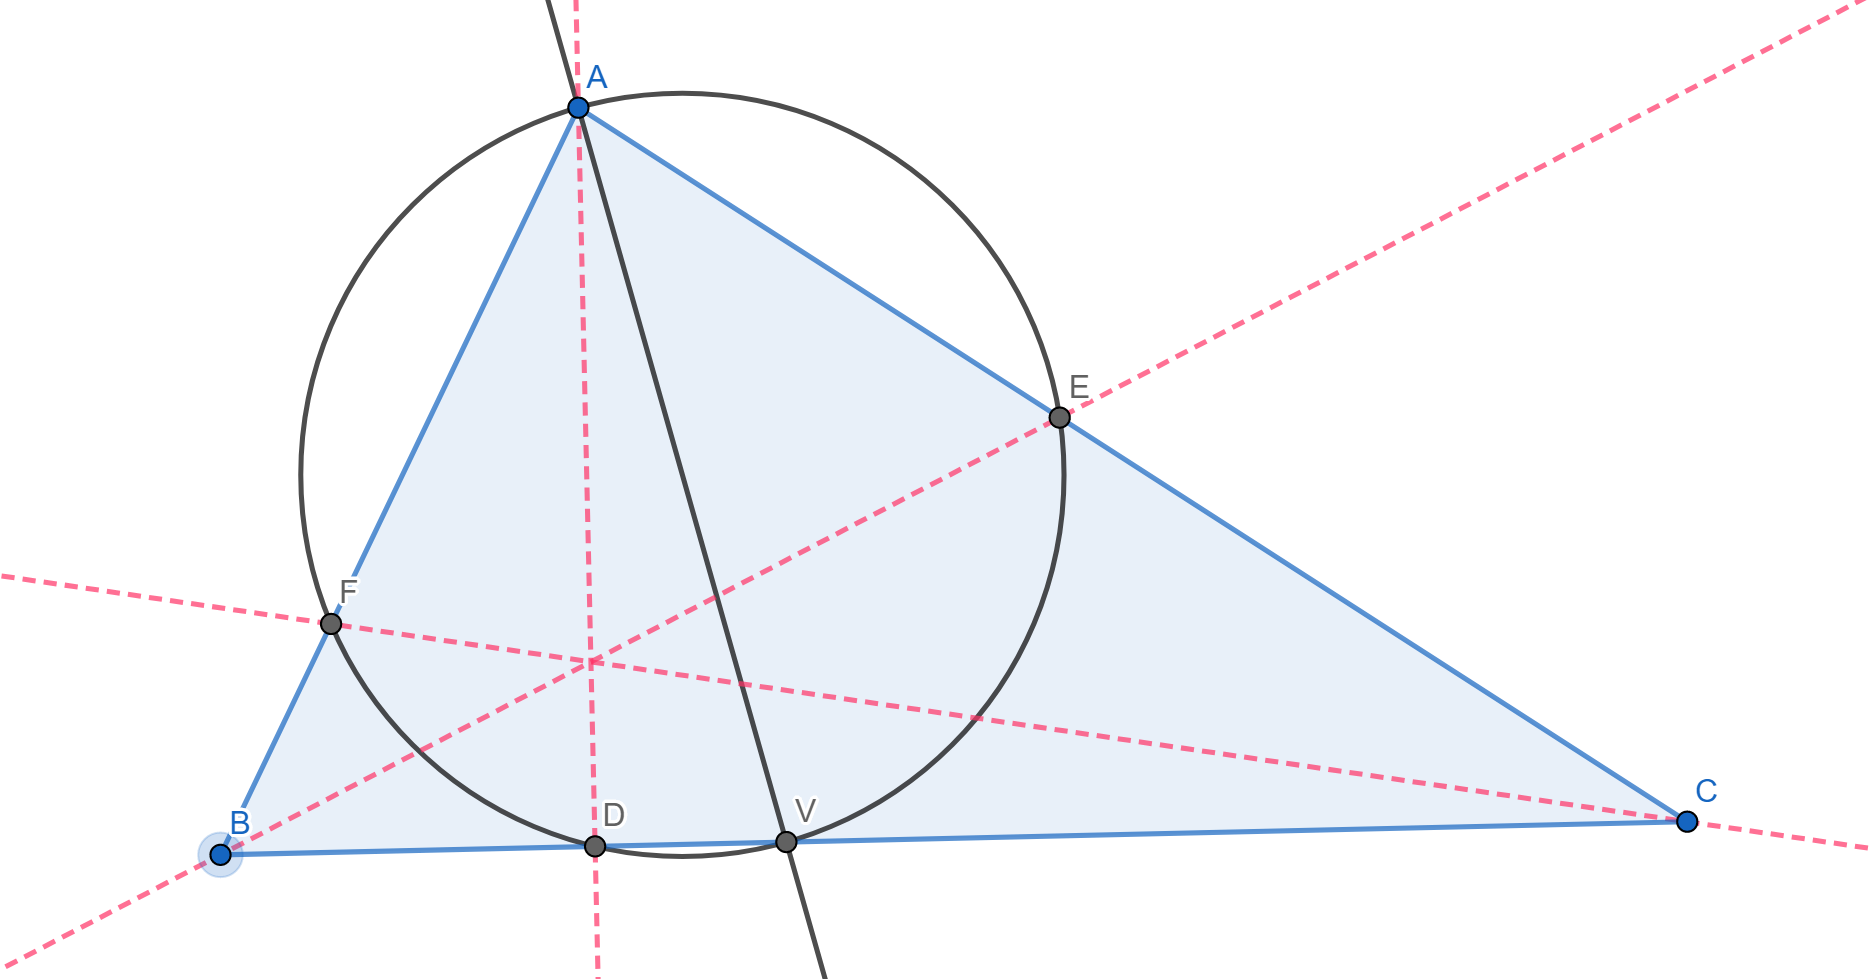
\includegraphics[scale=0.2]{JT1.png}
	\end{figure}
\end{sol}

\begin{sol}
	$(\implies)$ Llame $N = AD \cap FC$. Tenemos que $B, B, E$ son colineales. Ademas, tenemos las siguientes semejanzas (que salen de AAA + arco capaz): $\triangle AFN \simeq \triangle DNC \implies \frac{AF}{DC} = \frac{AN}{NC}, \triangle BAN \simeq \triangle DEN \implies \frac{AB}{ED} = \frac{AN}{NE}, \triangle BCN \simeq \triangle EFN \implies \frac{BC}{FE} = \frac{CN}{NE}$. Multiplicando todo da 
	\begin{align}
    \frac{AF\cdot DE \cdot BC}{DC \cdot AB \cdot FE} = \frac{AN\cdot NE \cdot CN}{NC\cdot AN \cdot NE} = 1 \hspace{0.2cm} \square \label{Eq5}
	\end{align}
	$(\impliedby)$ Sea $E'$ la intersecci\'on de la recta $BN$ con el circunc\'irculo del hex\'agono. Queremos probar que $E' = E$. Como la ecuaci\'on \ref{Eq5} es satisfecha por ambos puntos, concluimos que
	\begin{align}
	\frac{FE}{ED} = \frac{FE'}{E'D}
	\end{align}
	Pero veamos que si $E' \neq E \implies 	\frac{FE}{ED} \neq \frac{FE'}{E'D}$, debido a que $FE' > FE \iff E'D < ED$. Por lo tanto, $E'=E \hspace{0.2cm} \square$.
\end{sol}

\begin{sol}
	Sea $H = AB = \cap PC, I = AP \cap CE, G = PA \cap FC$. Primero, veamos que los tri\'angulos $\triangle AFC \simeq \triangle GFA \simeq \triangle GAC$, por AAA ($\angle{GAF} = \angle{FCA}$ por ser un angulo tangente). De estas semejanzas obtenemos:
	\begin{align}
	\frac{GF}{FA} = \frac{GA}{AC}, \frac{FC}{FA} = \frac{AC}{GA} \implies \frac{GF}{FC} = \bigg(\frac{GA}{AC}\bigg)^{2}
	\end{align}
	De manera an\'aloga, usando las semejanzas $\triangle IAC \simeq \triangle IEA \simeq \triangle EAC$ vamos a obtener que 
	\begin{align}
	\frac{IE}{EC} = \bigg(\frac{IA}{AC}\bigg)^{2}
	\end{align}
	Combinando las \'ultimas dos ecuaciones obtenemos que
	\begin{align}
	\frac{GF}{FC} \cdot \frac{IE}{EC} = \bigg(\frac{GA}{IA}\bigg)^{2} \label{EQ6}
	\end{align}
	Observe ahora que como $AM = MC$, y $AH, CI, PM$ son concurrentes por definici\'on, tenemos que, debido al teorema de Thales,
	\begin{align}
	\frac{IP \cdot AM \cdot CH}{AI \cdot MC \cdot PH} = 1 \implies IH \parallel AC 
	\end{align}
	Entonces, usando el teorema de thales en $\triangle APC \implies AI = \frac{IP \cdot HC}{PH}$. Tenemos tambi\'en que $AH \parallel CG \implies GA = \frac{AP \cdot HC}{PH}$
	Sigue entonces que
	\begin{align}
	\bigg(\frac{GA}{IA}\bigg)^{2} = \bigg(\frac{AP \cdot HC}{PH} \cdot \frac{PH}{IP \cdot HC}\bigg)^{2} = \bigg(\frac{AP}{IP}\bigg)^{2} = \frac{PG}{IP} \label{EQ7}
	\end{align}
	
	La \'ultima igualdad sigue de usar Teorema de Thales. En el tri\'angulo $\triangle GCP \implies GP = \frac{PA \cdot PC}{PH}$, y en $\triangle APC \implies \frac{AP}{IP} = \frac{PC}{PH} \implies GP = \frac{AP^{2}}{IP}$.
	
	Usando entonces (\ref{EQ6}) + (\ref{EQ7}) obtenemos que
	\begin{align}
	\frac{GF}{FC} \cdot \frac{IE}{EC} \cdot \frac{IP}{GP} = 1 
	\end{align}
	Y por el teorema de Menelao, los puntos P, E y F son colineales.
	\begin{figure}[h!] 
		\centering
		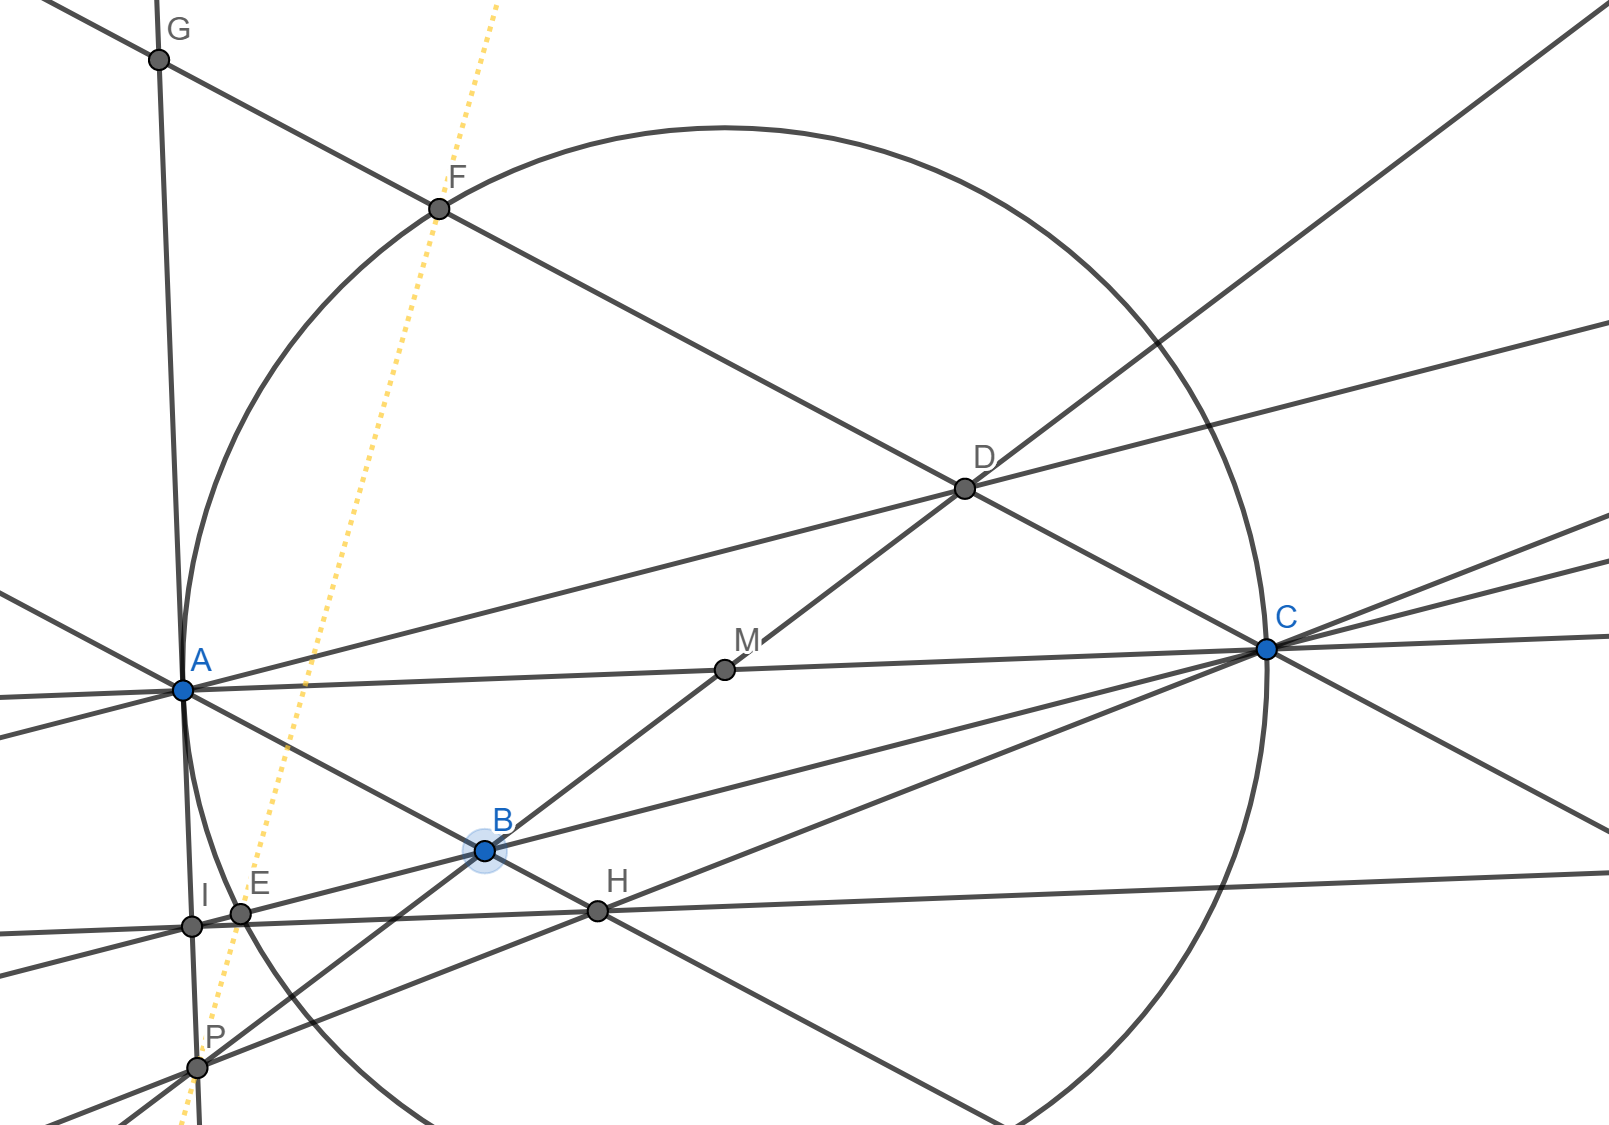
\includegraphics[scale=0.4]{JT2.png}
	\end{figure}
\end{sol}

\begin{sol}
	Es un hecho conocido que $\angle{APO} + \angle{ABP} = 90^{\circ}$. Por arco capaz tenemos $\angle{APD} = \angle{ACD}$. Sea $M = OP \cap DC$ Entonces $\angle{PMC} = \angle{MPC} + \angle{PCM} = 90^{\circ}$, que implica que $P, M, H$ y $O$ son colineales. 
\end{sol}

\begin{sol}
	Listemos las igualdades obtenidas usando potencia de un punto:
	\begin{align}
	BL \cdot BL' &= BN \cdot BN' \\
	CL \cdot CL' &= CM' \cdot CM \\
	AM \cdot AM' & = AN \cdot AN' 
	\end{align}
	Escrito en otras formas, tenemos 
	\begin{align}
	\frac{BL}{BN}&= \frac{BN'}{BL'} \\
	\frac{CL}{CM}&= \frac{CM'}{CL'} \\
	\frac{AM}{AN}&= \frac{AN'}{AM'} 
	\end{align}
	Multiplicando las tres ecuaciones, sigue que
	\begin{align}
	1 = \frac{BL}{BN}\cdot \frac{CM}{CL} \cdot \frac{AM}{AN} = \frac{BN'}{BL'} \cdot \frac{CL'}{CM'} \cdot  \frac{AN'}{AM'}  \square
	\end{align}
\end{sol}

\begin{sol}
	Supongamos que $Q$ es el circuncentro del tri\'angulo $\triangle DEF$, donde los puntos $D, E, F$ son los puntos medios de $MN, KM, NK$. Si $I$ es el incentro de $\triangle ABC$, tenemos que $I$ es el circuncentro de $MNK$. Tambi\'en $Q$ es el centro de la circunferencia de los nueve puntos de $MNK$. Por lo tanto, $IQ$ es la recta de Euler de $MNK$, y el ortocentro $H$ de $MNK$ pertenece a la recta $IQ$. Defina $\Omega$ como siendo el circunc\'irculo de ABC, $B' = BI \cap \Omega$, y an\'alogamente defina $A', C'$. Observe que los tri\'angulos $\triangle MNK$ y $\triangle A'B'C'$ son semejantes porque sus tres lados son paralelos. Es decir, existe un centro de homotecia que lleva $MNK$ a $A'B'C'$. Este centro de Homotecia lleva adem\'as el circunc\'irculo de $\triangle MNK$ a $\Omega$. Por lo tanto esta homotecia lleva $I \to O$ y $H \to I$, debido a que $I$ es el ortocentro de $A'B'C'$, $H$ es el ortocentro de $MNK$, $I$ es el circuncentro de  $MNK$. Como la homotecia es lineal tenemos que $H$, $I$ y $O$ son colineales. Sigue que $Q$, $I$ y $O$ son colineales.
\end{sol}